\documentclass[11pt, a4paper]{article}
\usepackage[utf8x]{inputenc}
\usepackage[sort]{natbib}

\usepackage[spanish]{babel}
\usepackage{enumitem}
\usepackage{graphicx}
\usepackage{float}
\usepackage[linktoc=all]{hyperref}

\usepackage{etoolbox}

\usepackage{amsmath}
\usepackage{amssymb}
\usepackage{array}
\usepackage{gensymb}

\usepackage{fancyhdr}
\usepackage{multirow}
\usepackage{multicol}
\usepackage[table]{xcolor}
\usepackage{color}
\usepackage{colortbl}
\definecolor{lightgray}{gray}{0.9}
\setlength{\columnsep}{0.5cm}

\usepackage{tikz}
\usetikzlibrary{shapes.geometric, arrows}
\tikzstyle{problema} = [rectangle, rounded corners,  minimum width=3cm, minimum height=1cm,text centered, draw=black,fill={rgb:black,1;white,30}]
\tikzstyle{causa} = [rectangle, minimum width=3cm, minimum height=1cm, text centered, text width=4cm, draw=black, fill={rgb:black,0;white,10}]
\tikzstyle{nodo} = [diamond, minimum width=1cm, minimum height=1cm, text centered, draw=black, fill={rgb:black,0;white,10}]
\tikzstyle{arrow} = [thick,->,>=stealth]



%------------------- Dimensiones -------------------
\usepackage{geometry}
 \geometry{a4paper,total={170mm,257mm},left=15mm,right=15mm,top=20mm,}
%----------------------------------------------------

%------------------- Encabezado y Pie de pág -------------------
\pagestyle{fancy}
\fancyhf{}
\lhead{Electrónica de Potencia}
\rhead{TP9 : Driver de motor de induccion.} 
\rfoot{Página \thepage}
%----------------------------------------------------


%----------------------------- Documento -----------------------------------------------
\begin{document}
\begin{titlepage}
 \centering
	
\includegraphics[scale=0.80]{imagenes/LOGO.jpg} \par
 	\vspace{1cm}
 	{\scshape\LARGE Universidad Tecnológica Nacional \par}
 	{\scshape\large Facultad Regional de Córdoba \par}
 	\vspace{1cm}
	{\bfseries \Large Trabajo Práctico De Laboratorio $N^{\circ} 9$\par}
	{\bfseries \Large Driver de motor de inducion.\par}
 	\vspace{1.5cm}

	\begin{tabular}{ll}
		Alassia, Francisco		&	60861	\\
		Amaya, Matías			&	68284	\\
		Lamas, Matías			&	65536 	\\
		Navarro, Facundo		&	63809 	\\
		Veron, Misael			&	62628
	\end{tabular}
	
	\vspace{1cm}
	Curso: 5r2 \\
	Grupo $N^{\circ} 11$
 	\vfill
	{\bfseries \Large Electrónica de Potencia \par}

	\vspace{1.5cm}
	Docentes: \par
	Ing. Oros, Ramón \par
	Ing. Avramovich, Javier \par

 	\vfill
	{\large \today\par}
\end{titlepage}
	
	
\tableofcontents
\clearpage

\section{ Descripción del circuito}

El circuito es en lazo abierto.
El motor de AC está alimentado por un convertidor de AC del tipo SPWM, donde se puede obtener referencia de velocidad, como se muestra en la Fig.\ref{vel}.

La carga mecánica está caracterizada por un escalón de carga TL, con un valor inicial de 0Nm, y en 1s pasa a 10Nm, como muestra la fig.\ref{par}.


\section{Objetivos}

Ejecute la simulación (Matlab), archivo \textbf{"induction motor drive.mdl"}.\\
Observe en el osciloscopio la velocidad y el par temporales.
Observe en el osciloscopio las corrientes ir, is y la tensión Vab.


\subsection*{ Mediciones a realizar}

\subsubsection*{ Realice el siguiente análisis:}


\begin{itemize}

\item[a] Interprete el circuito, la señal de entrada y la variación de par de carga.

\item[b]  Corra el circuito de Simulink.

\item[c] Imprima los resultados.

\item[d] Interprete los resultados, en base a la variación de la señal de referencia y variación del par de carga TL.

\item[e] Analice la variación de Vab.


\end{itemize}




\subsubsection*{ Conclusiones:}

\textbf{Escriba las siguientes conclusiones}

\begin{itemize}
\item[a] Acerca del modo de arranque.
\item[b] Acerca de la ecuación general de par $Te=TL+J\cdot \dfrac{d(wm)}{dt} $
\item[c] Acerca de la velocidad y el par en función del tiempo.
\item[d] Generales (otros).

\end{itemize}






\newpage

\section{Introducción}
En el siguiente práctico se lleva a cabo la simulación de un control a lazo abierto de un motor de inducción trifásico, a través de un inversor para  regular la velocidad del mismo.\\
La simulación consiste en aplicar una señal de velocidad de control y observar el comportamiento del motor en base a esta velocidad, a 1 $s$ de haber arrancado la simulación se produce la variación del par de carga y a 1.4 $s$ retoma su valor inicial. Luego,  a 1.6 $s$ se produce una variación de la velocidad de referencia disminuyendo un $10\%$ de la misma.\\
En las siguientes figuras se pueden observar el circuito de simulación y las señales de velocidad de referencia y par de carga.\\

\begin{figure}[H]
\centering
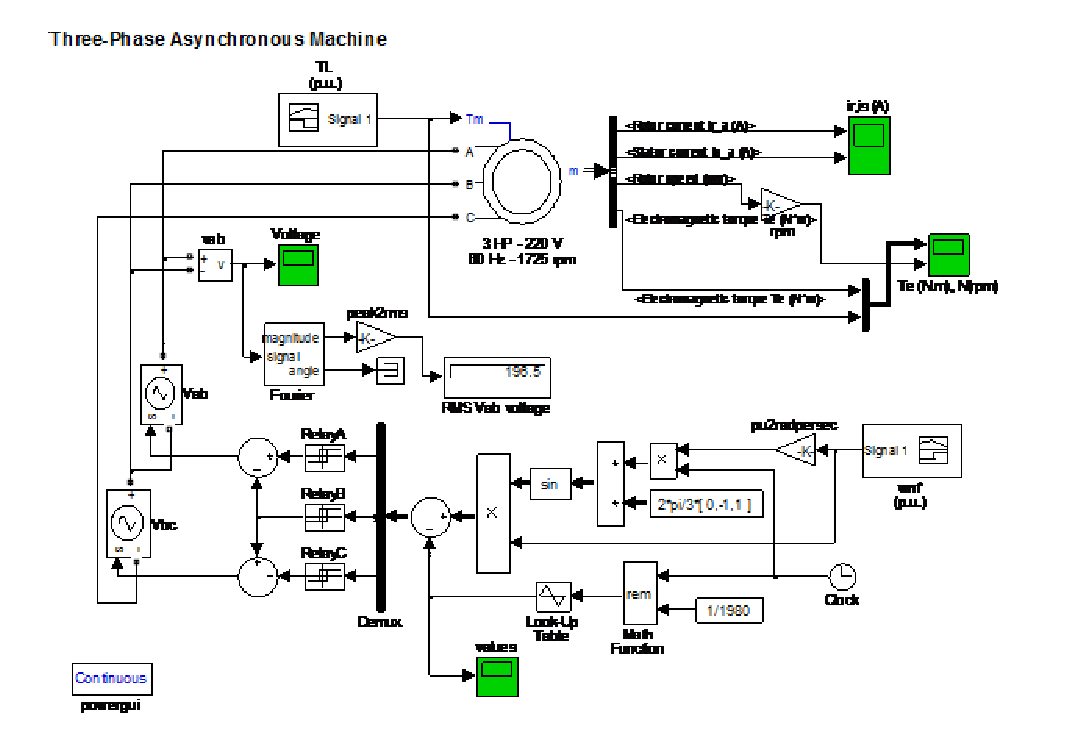
\includegraphics[scale=0.8]{imagenes/circuito}
\caption{Circuito de simulación}
\label{circuito}
\end{figure}

\begin{figure}[H]
\centering
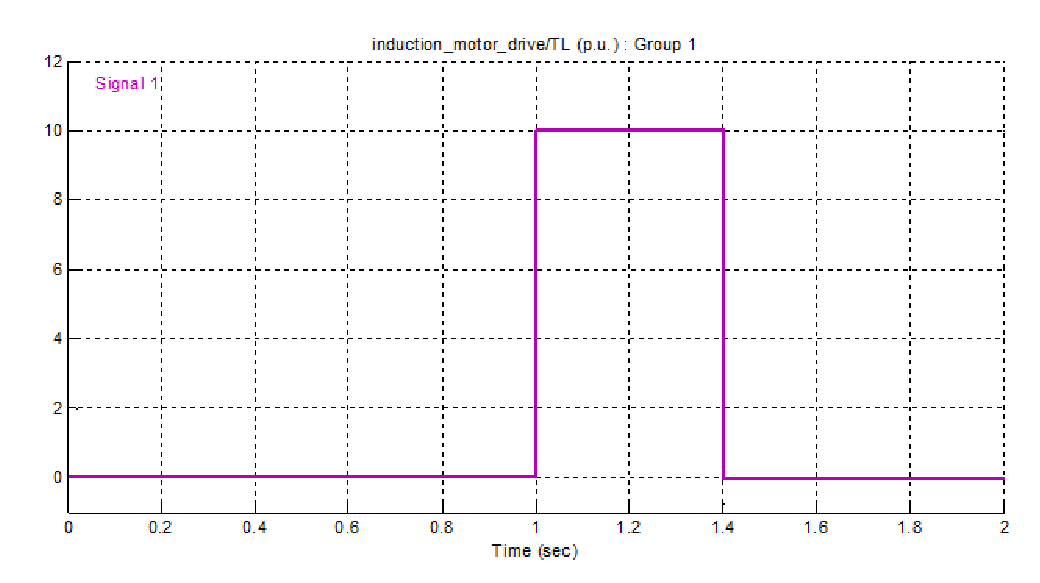
\includegraphics[scale=0.75]{imagenes/par}
\caption{Par de carga}
\label{par}
\end{figure}

\begin{figure}[H]
\centering
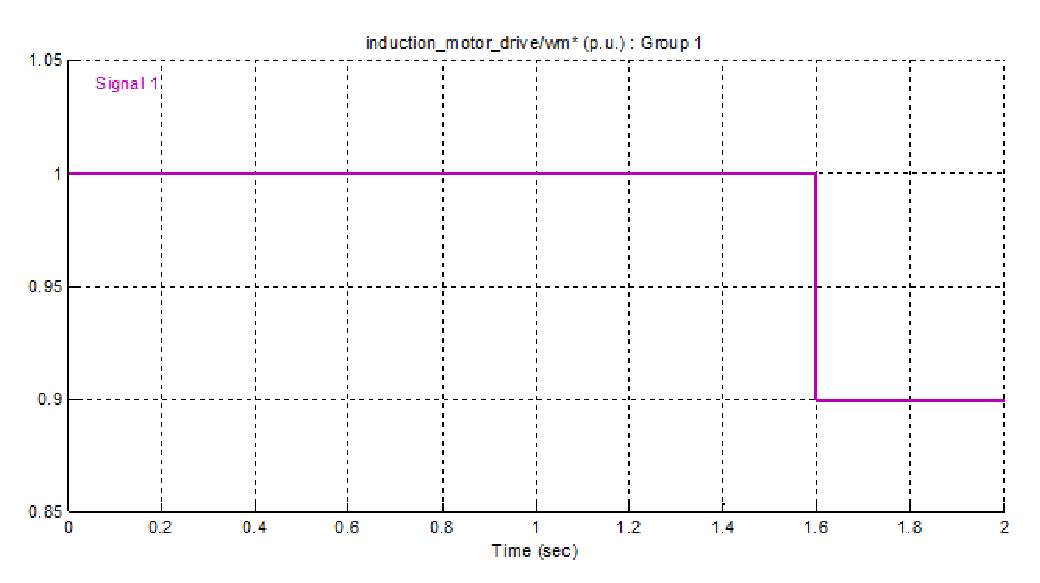
\includegraphics[scale=0.75]{imagenes/velocidad}
\caption{Velocidad de referencia}
\label{vel}
\end{figure}


\newpage
\section{Simulación}
A continuación se muestran las capturas del osciloscopio del simulador \emph{Simulink}.\\

\begin{figure}[H]
\centering
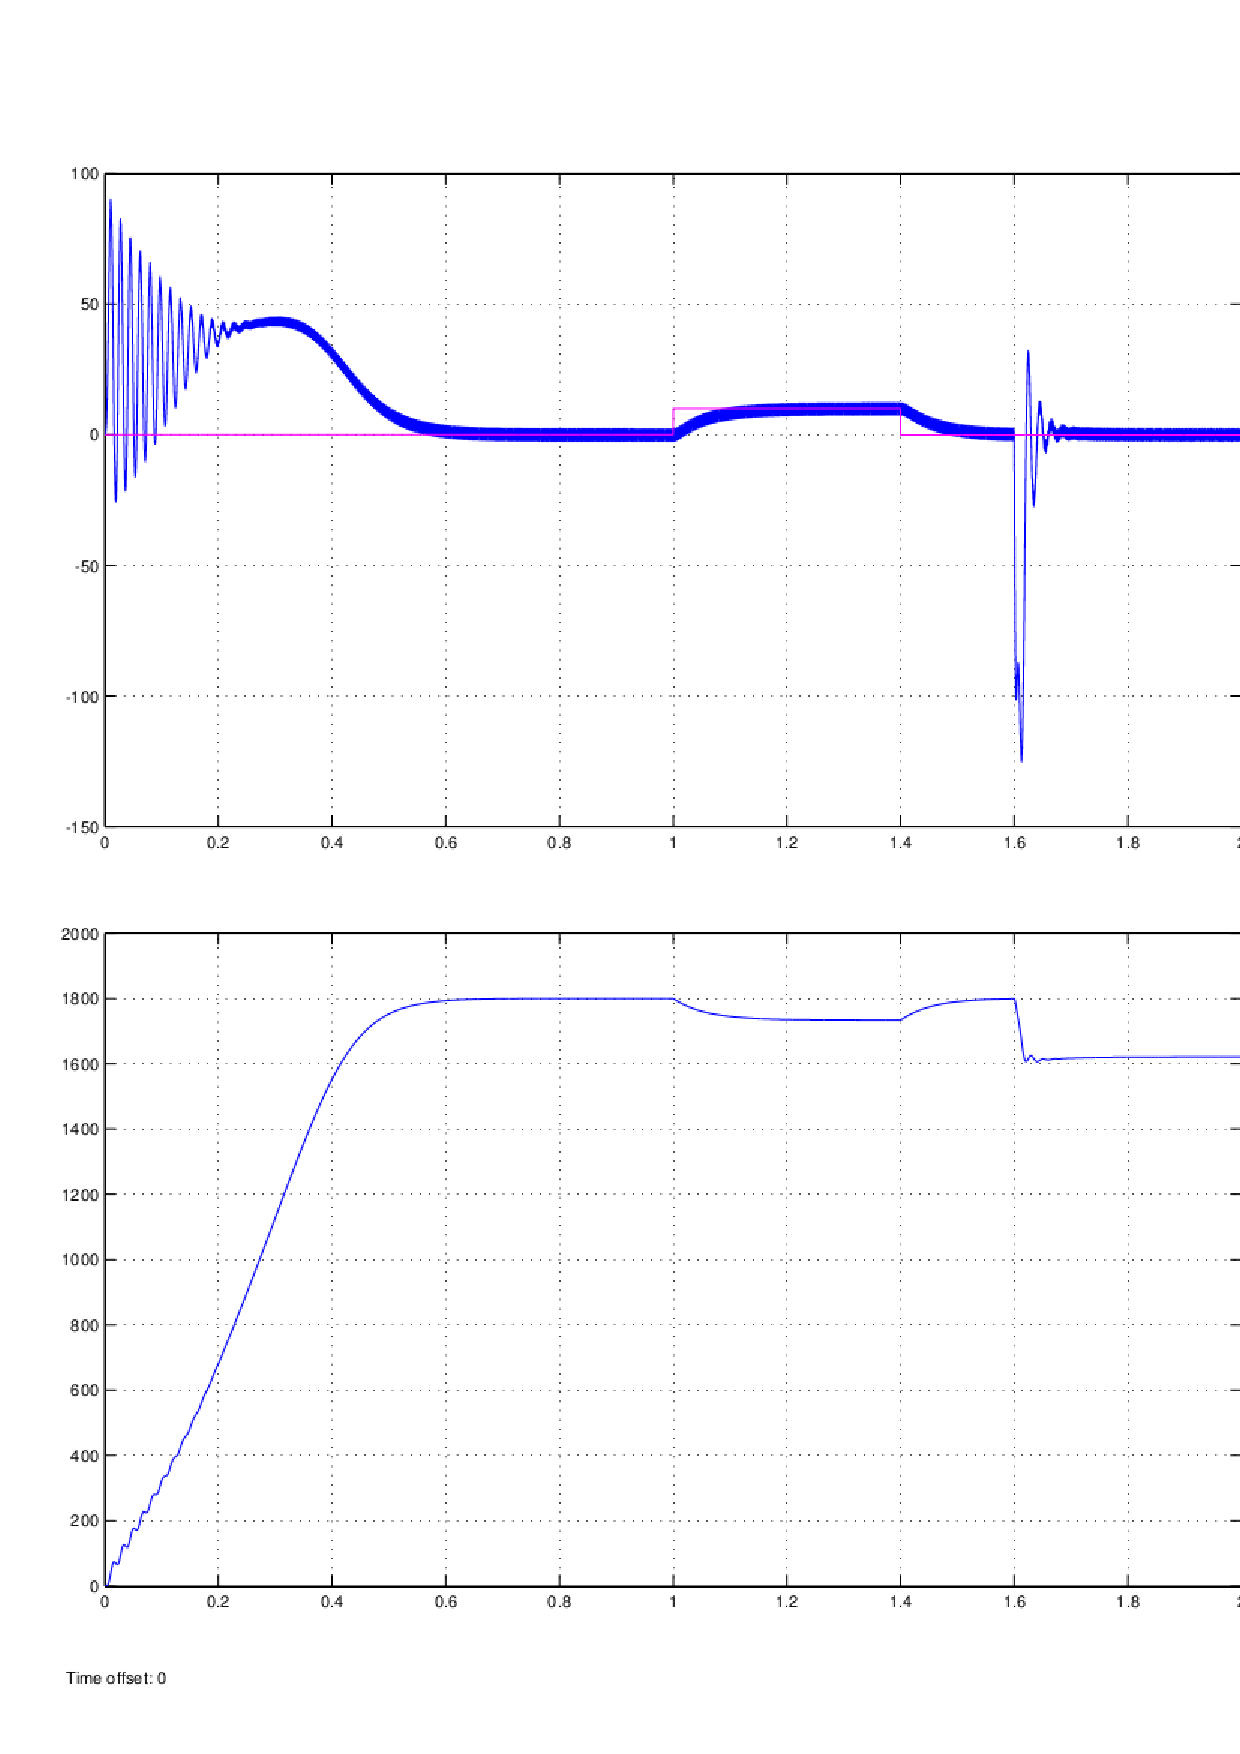
\includegraphics[scale=0.8]{imagenes/parvel}
\caption{Par y velocidad del motor}
\label{parvel}
\end{figure}

\begin{figure}[H]
\centering
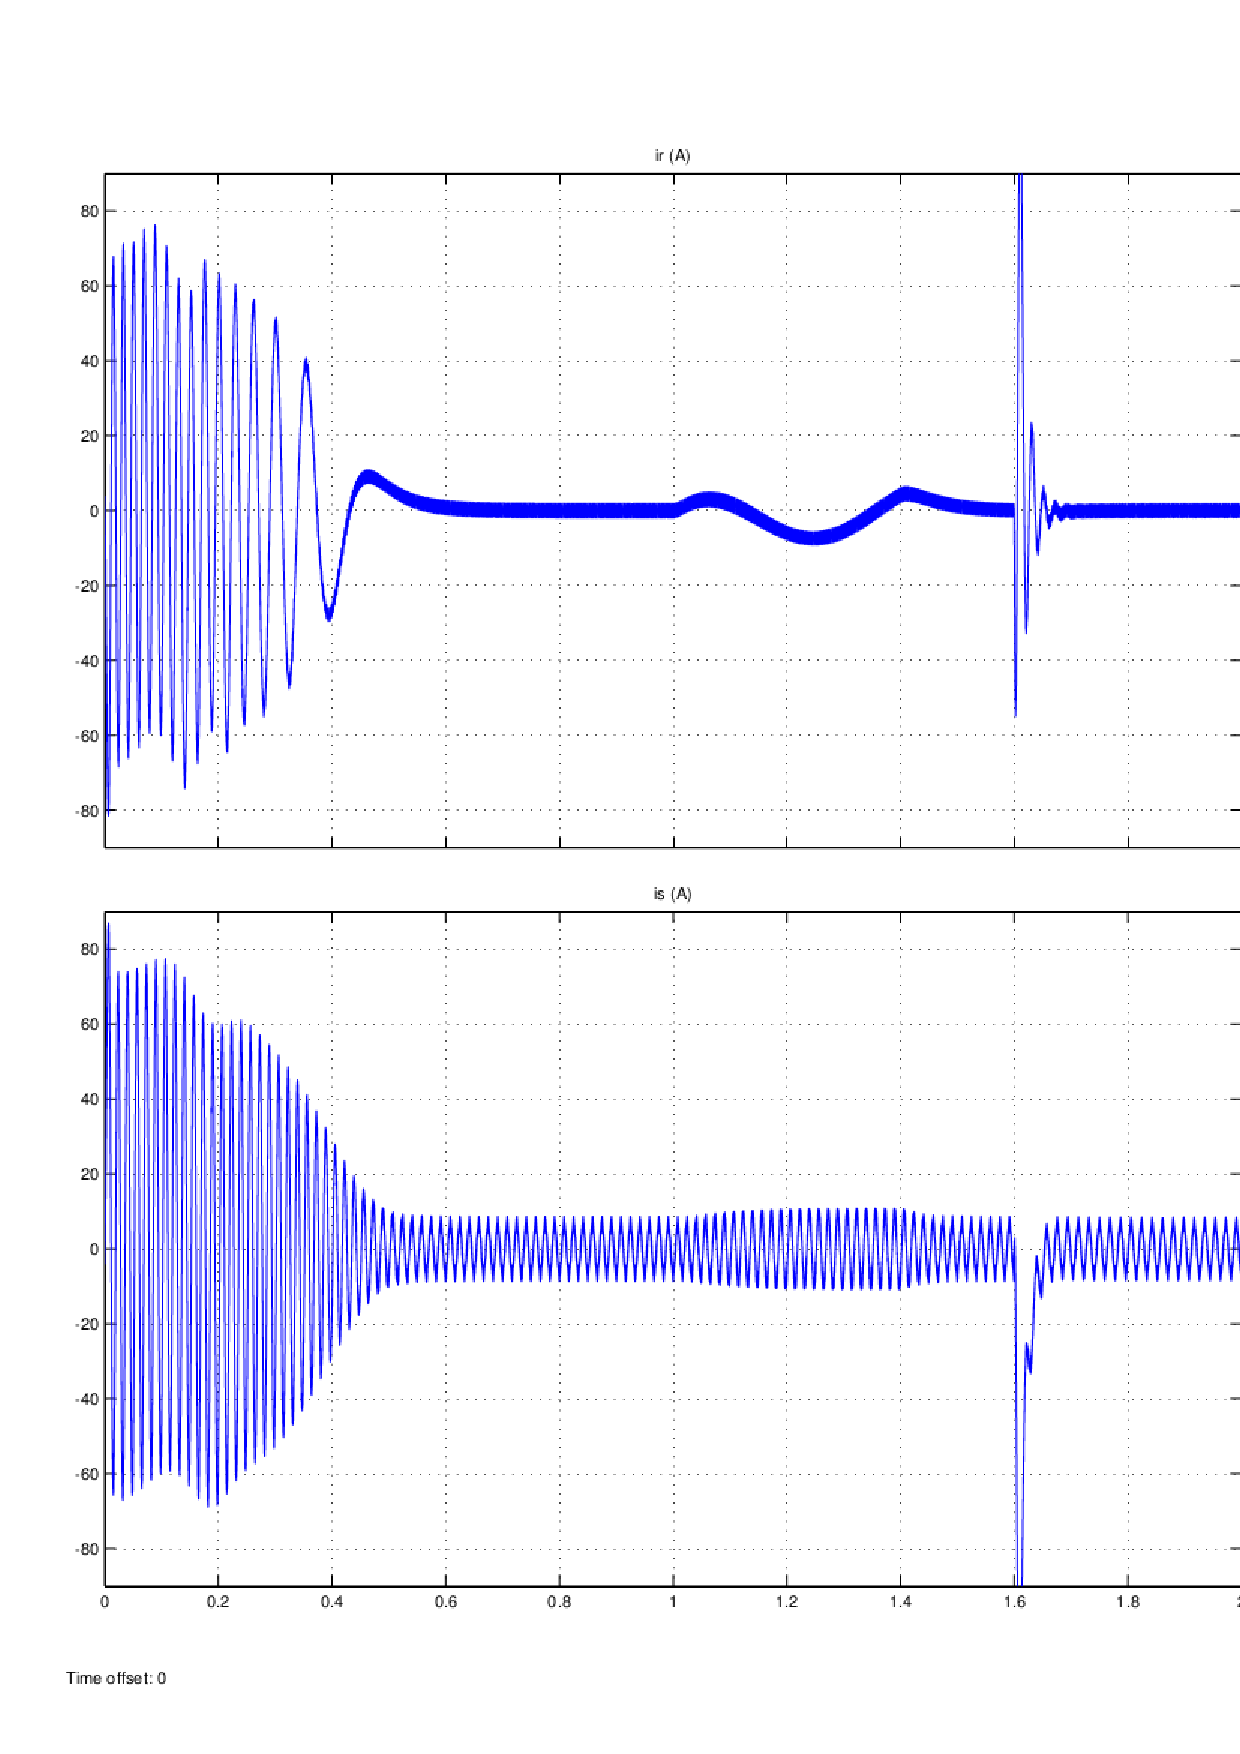
\includegraphics[scale=0.8]{imagenes/corrientes}
\caption{Corrientes de rotor y estator}
\label{corrientes}
\end{figure}

\begin{figure}[H]
\centering
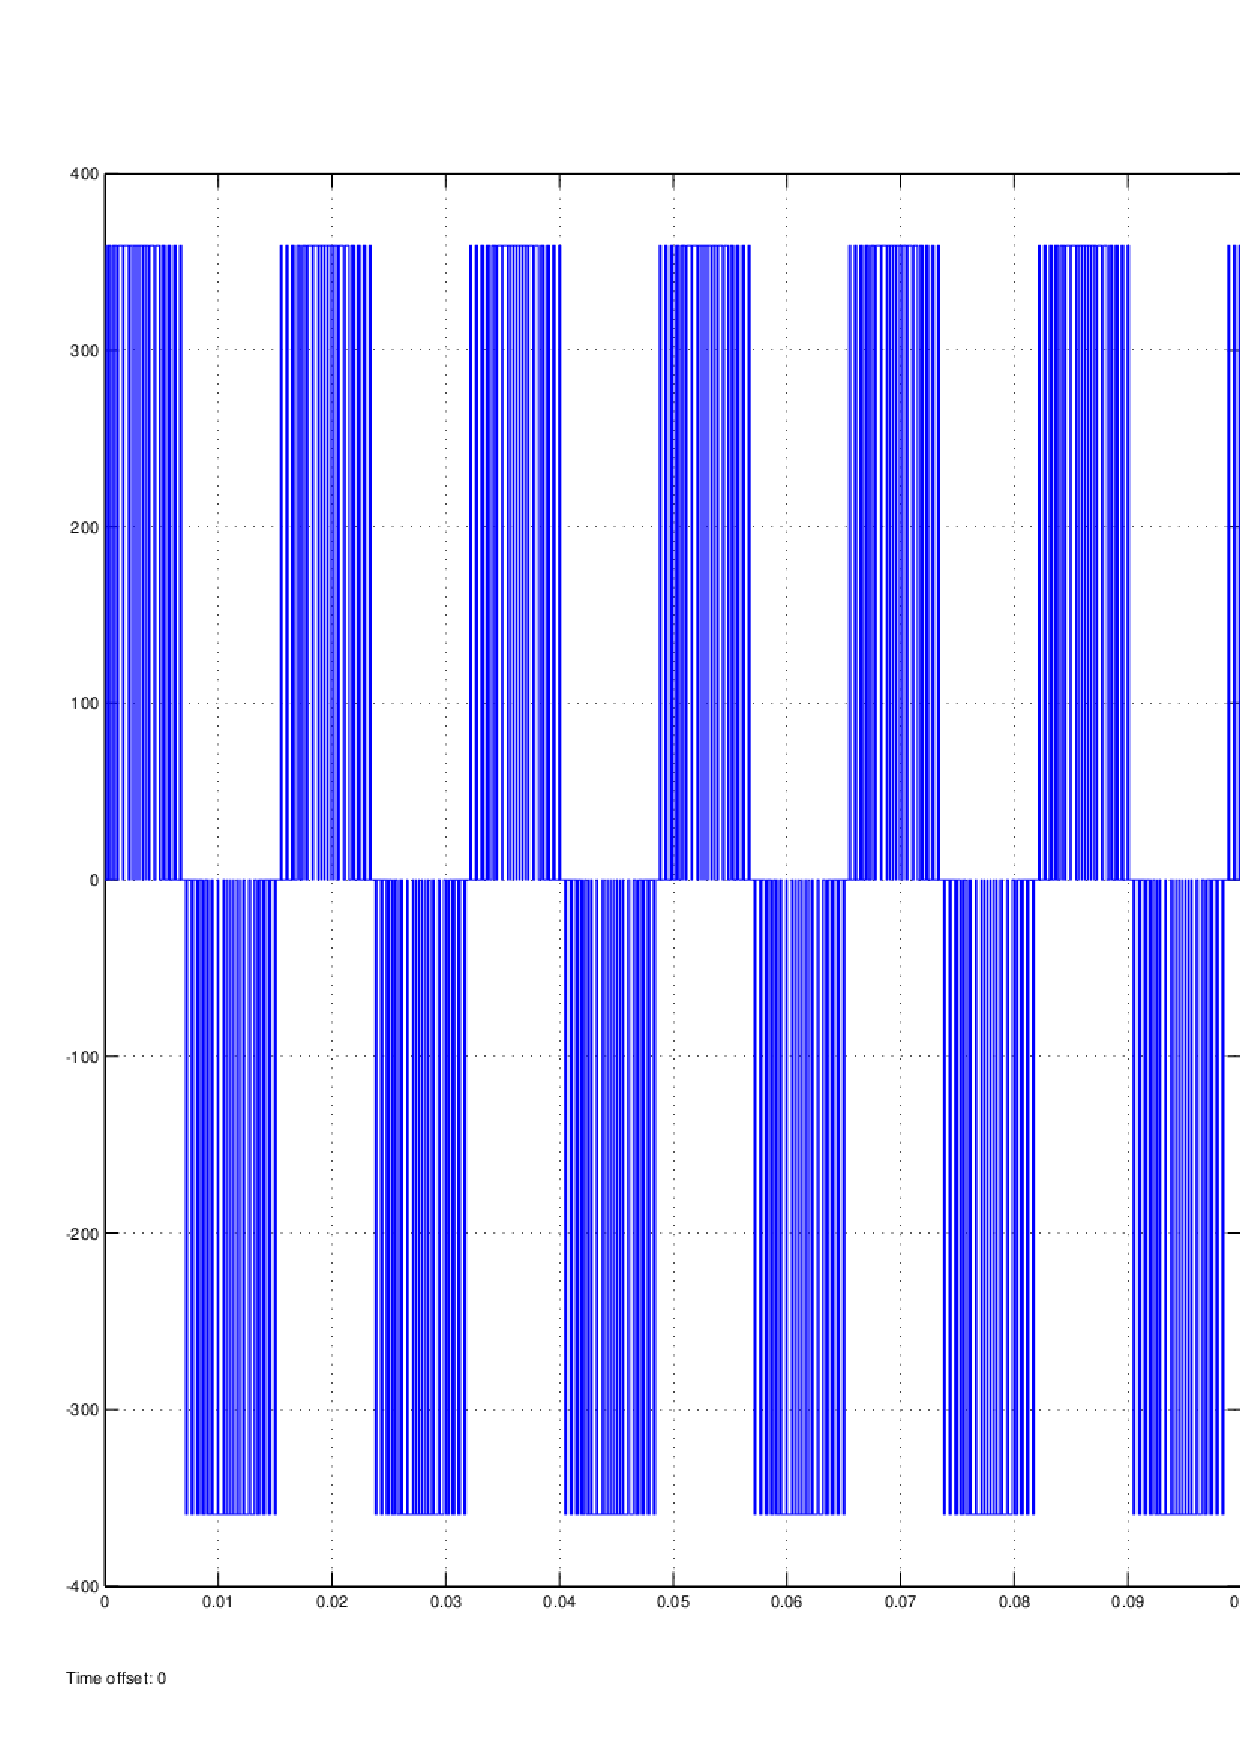
\includegraphics[scale=0.5]{imagenes/tension}
\caption{Tensión de alimentación del motor}
\label{tension}
\end{figure}


Como se puede observar en la Fig.\ref{parvel}, al inicio de la simulación el sistema tiene que vencer la inercia del motor, por lo cuál  se produce un gran pico de corriente, tanto en el rotor como en el estator, y esto produce que la velocidad del motor se vaya incremetando linealmente hasta la de referencia, como ésta es 1 la velocidad de salida es la máxima del motor ( $1800 rpm$), a su vez como el par generado por el motor es proporcional a la corriente, se observa como se produce la variación del mismo hasta estabilizarse (aprox $0.6 s$).

\vspace*{0.5cm}
Luego se observa ,en 1 $s$,  una variación en el par generado por el motor, la corriente de estator (is) y la de rotor (ir), esto se debe a la variación del par de carga, que pasa de 0 a un valor de 10 $N.m$. Se puede apreciar como se genera un retardo en el par generado por el motor, al momento exacto del cambio del par, con una cierta pendiente de crecimiento y una de decrecimiento cuando el valor del par de carga vuelve a su valor inicial.
Esto produce un retardo en el par generado por el motor. A su vez se observa que la velocidad del motor disminuye al aplicar el par de carga distinto y vuelve a su valor inicial al mismo tiempo que el par generado por el motor.
\vspace*{0.5cm}
Una vez estabilizado  nuevamente se observa como a un valor de 1.6 $s$ la velocidad del motor disminuye en un $10\%$, esto es lo que se denomina un \textit{frenado del motor}, generando una gran variación de corriente, tanto en el estator como en el rotor, y produce una variación en el par generado por el motor.\\
Como se ve en la Fig.\ref{tension}. no se produce una variación en la tensión de alimentación, pero luego se realizó un barrido de  mas tiempo de dicho valor y se ve como la tensión varía a los $1.6 s$ en donde la referencia de velocidad en el inversor cambió de valor, esto se puede observar en la Fig. \ref{zoomte}. como varía la tensión que llega al motor.% y el valor de la tensión RMS medida en el mismo.\\

\begin{figure}[H]
\centering
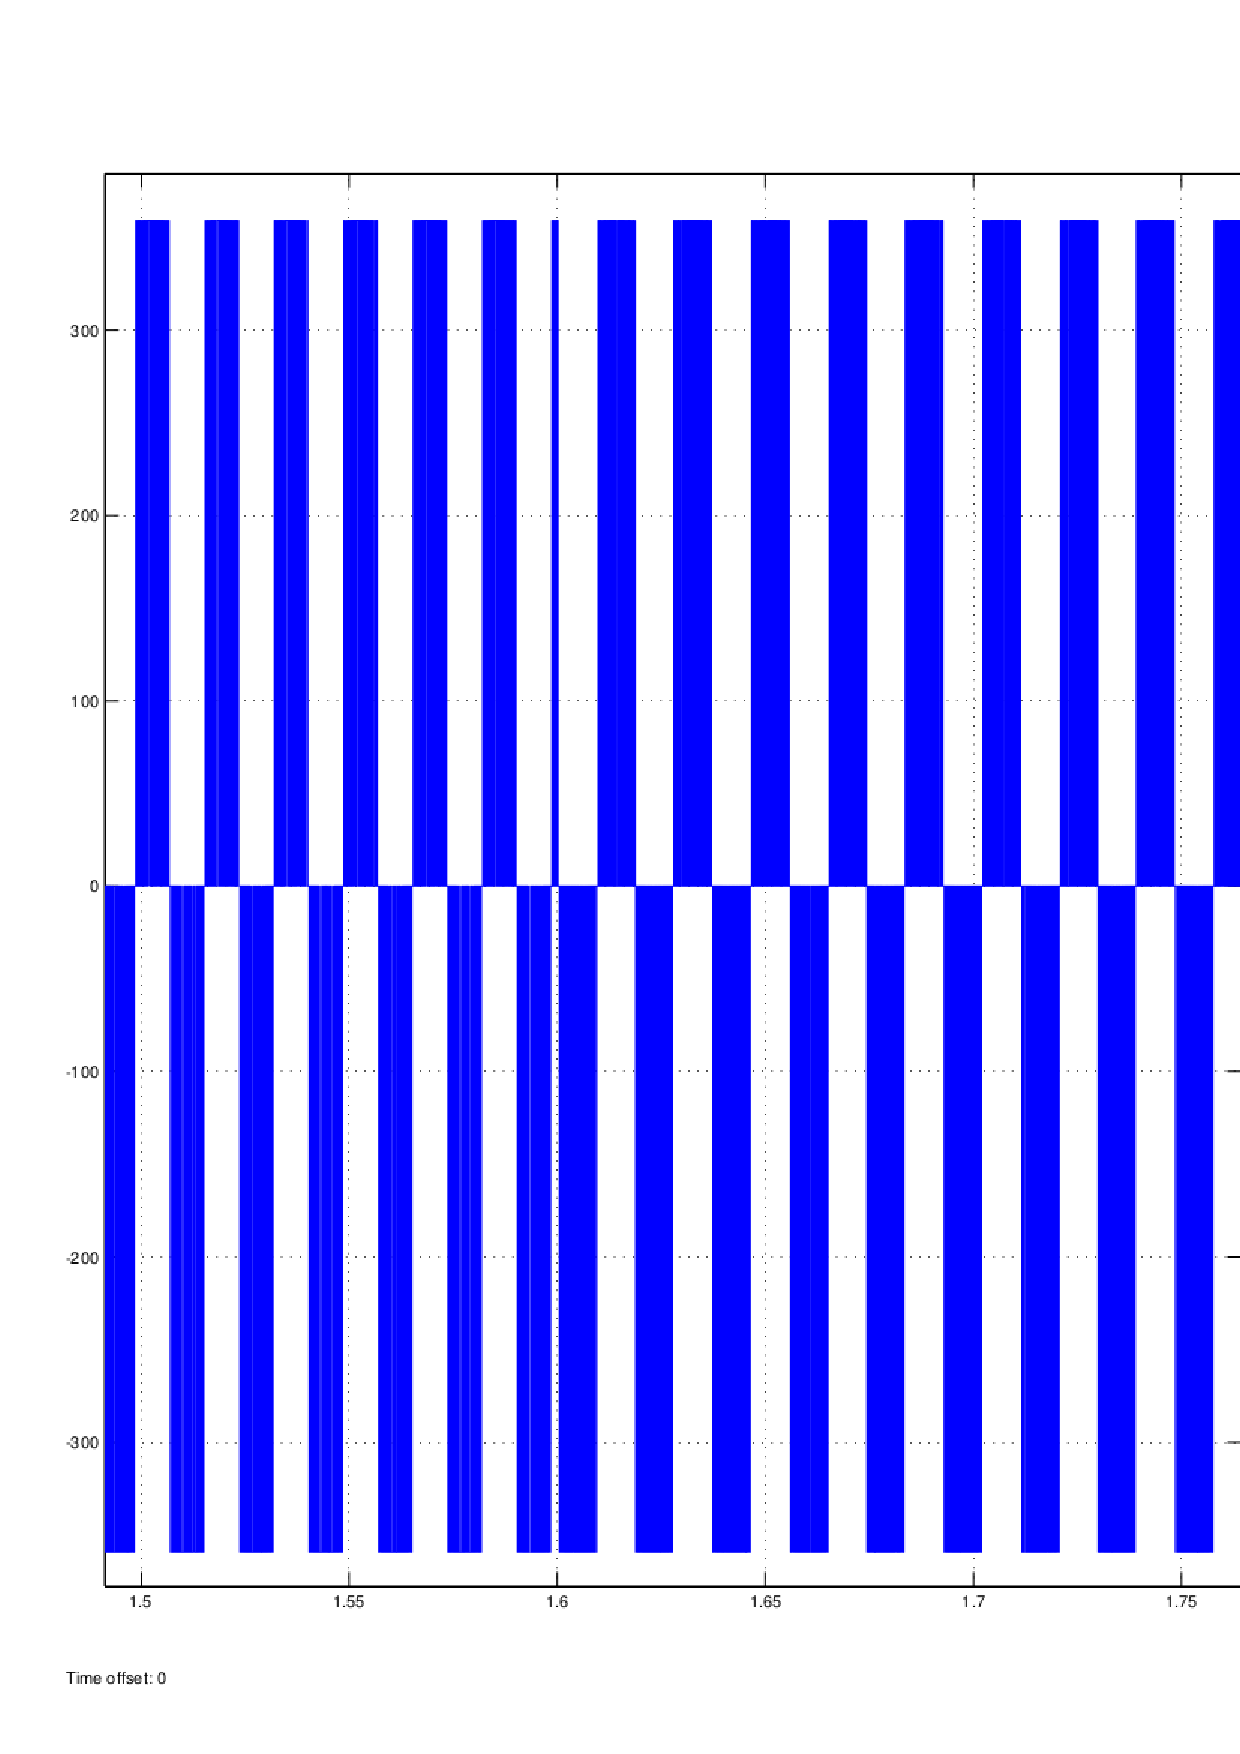
\includegraphics[scale=0.5]{imagenes/zoomtension}
\caption{Variación de tensión provocada por variación de la velocidad de referencia}
\label{zoomte}
\end{figure}


\newpage

\section{Conclusión} 


\begin{itemize}
\item[a] \textbf{Acerca del modo de arranque}\\
En el instante de arranque se aplica una tensión pequeña en el motor, de
manera que se produce un arranque suave, aumentando la velocidad del rotor
de una manera lenta. Luego al incrementarse el valor de dicho escalón se
producen oscilaciones por un intervalo de tiempo corto hasta que el motor
llega rápidamente a las condiciones de velocidad establecidas por la referencia (régimen
permanente).

\item[b] \textbf{Acerca de la ecuación general de par  $Te=TL+J\cdot \dfrac{d(wm)}{dt} $}\\
Esta ecuación vincula la carga aplicada al motor siendo
proporcional a esta y también  proporcional a la variación de aceleración
angular. El par motor desarrollado debe ser igual al par de carga del motor
más la inercia total del motor (inercia propia del motor más la inercia
externa reflejada en el eje del motor) por la aceleración angular del mismo.

\item[c] \textbf{Acerca de la relación velocidad/amplitud}\\
La variación de amplitud del circuito SPWM provoca una variación
proporcional de velocidad en el motor, debido al aumento de la tensión
eficaz en cada devanado y la corriente de los mismos.
\end{itemize}

















\end{document}
